\documentclass{ximera}



% MATH -----------------------------------------------------------
\newcommand{\nats}{\mathbb N}
\newcommand{\ints}{\mathbb Z}
\newcommand{\rats}{\mathbb Q}
\newcommand{\reals}{\mathbb R}
\newcommand{\complex}{\mathbb C}
\newcommand{\powerset}{\mathscr P}

%-------------------------------------------------------------


\begin{document}
\begin{abstract}
 \end{abstract}

    \title{2nd Order Applications, Part II (Circuits)}
    
    \maketitle

 There are many applications of 2nd order differential equations, particularly 2nd order linear.  We take a look at a couple.\\

 RLC Circuits: An RLC circuit is one that includes a voltage source of voltage $V(t)$ (SI units of volts) as a function of time, a resistor of resistance $R>0$ (SI units ohms), a coiled wire inductor of inductance $L>0$ (SI units henries), and a plate capacitor of capacitance $C>0$ (SI units farads).\\


 \begin{figure}[h]
\centering
 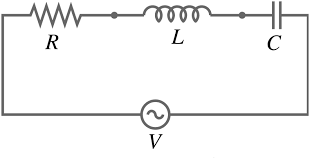
\includegraphics[scale=0.8]{RLC.png}
\caption{An RLC circuit}
 \end{figure}


 Let $Q(t)$ be the charge (SI units of coulombs)  on one plate of the capacitor at time $t$.   Then $I(t)=\dfrac{dQ}{dt}$ is the electrical current (SI units of amps) in the circuit (flowing towards one plate if positive and the opposite direction if negative).   From physics we have the following basic laws for the change in voltage across each circuit component:

\begin{itemize}
\item Resistor: $V=IR$\\
\item Inductor: $V=L\dfrac{dI}{dt}$\\
\item Capacitor: $V=\dfrac{Q}{C}$\\
\end{itemize}


Kirchhoff’s law that says that the voltage change across any two points has to be independent of the path used to travel between the two points.  Hence $$L\dfrac{dI}{dt}+IR+\dfrac{Q(t)}{C}=V(t).$$

\vspace{0.5cm}

 As $I=Q'$, this can be rewritten as \framebox{$\displaystyle LQ''+RQ'+\dfrac{1}{C}Q=V(t)$}.\\

By differentiating both sides, we can also express it in terms of current:  \framebox{$L I''+R I'+\dfrac{1}{C}I=V'(t)$}.\\



 For an alternating current voltage source $V (t) = E \sin{(\omega t)}$ the differential equation becomes
 $$ LI''(t) + RI'(t) + \dfrac{1}{C}I(t) = \omega E\cos{(\omega t)}.$$


\bigskip

 Let's find the general solution of this differential equation.  The complementary equation has a characteristic polynomial of $Lx^{2}+Rx+1/C=0$  which has roots at $$x=\dfrac{-R\pm \sqrt{R^{2}-4L/C}}{2L}=r_{1},r_{2}.$$

\bigskip

 Then the general solution to the complementary equation is either $I=c_{1}e^{r_{1}t}+c_{2}e^{r_{2}t}$ if  \\ \\$R> 2\sqrt{L/C}$ (overdamped)   or $I=(c_{1}+c_{2}t)e^{-\frac{R}{2L}t}$ if $R= 2\sqrt{L/C}$ (critically damped) \\  \\  or $I=e^{-\frac{R}{2L}t}\left[c_{1}\cos{\left(\dfrac{\sqrt{4L/C-R^{2}}}{2L}t\right)}+c_{2}\sin{\left(\dfrac{\sqrt{4L/C-R^{2}}}{2L}t\right)}\right]$ if $R< 2\sqrt{L/C}$ (underdamped).   In each case the complementary solution decays towards $0$ as $t\rightarrow \infty$.

\bigskip


 The method of undetermined coefficients, where we guess a particular solution of the form $I_{P}=A\cos{(\omega t)}+B\sin{(\omega t)}$,  yields (the viewer is left to check the details) \\ \\  $$A=-\dfrac{\omega E(L\omega^{2}-1/C)}{R^{2}\omega^{2}+(L\omega^{2}-1/C)^{2}}\mbox{ and }B=\dfrac{R\omega^{2} E}{R^{2}\omega^{2}+(L\omega^{2}-1/C)^{2}}.$$

\bigskip

 Putting the solutions together and imposing initial conditions allows us to solve for the current given any RLC circuit with any such voltage source and initial conditions.

\vspace{1cm}

 For example, suppose we have an RLC circuit where the resistance is $R=600$ ohms, the capacitance is $C=0.000001$ farads, the inductance is $L=0.25$ henries, and the voltage source is $V(t)=120\sin{(120\pi t)}$ volts.

\bigskip

  With these values $R<2\sqrt{L/C}$, $A\approx 0.0445$ and $B\approx 0.0104$.  So the general solution is \\ \\ $$I(t)\approx 0.0445\cos{(120\pi t)}+0.0104\sin{(120\pi t)}+e^{-1200t}\left[c_{1}\cos{\left(1600t\right)}+c_{2}\sin{\left(1600t\right)}\right].$$


 Then given initial conditions we can find $c_{1}$ and $c_{2}$ for a solution of the above form, called a \textbf{transient solution}, since the part of the solution involving $c_{1}$ and $c_{2}$ decays away quickly as $t\rightarrow \infty$.  In the long run the current approaches the \textbf{steady state} solution of \\ $I(t)\approx 0.0445\cos{(120\pi t)}+0.0104\sin{(120\pi t)}$.


\end{document}